\documentclass[10pt]{article}
\usepackage{icmlko}

\icmlmeta{IP 파운데이션 월드모델}{172}{분모를 맞추니 조건화가 사라졌다}{노트 171이 만든 뒤집힘이 조건화였는지 확인했다. 맞았다 --- 그리고 열여덟 노트짜리 흐름이 여기서 닫힌다}

\begin{document}

\twocolumn[
\icmlheader

\begin{abstract}
노트 171에서 걸음 불변 칸의 정확도가 판 $\rho$ 와 $+$0.564로 붙어 다른
잣대 셋과 반대 방향이었고, 그것을 ``분모가 다른 두 수를 견준 탓''으로
읽었다. 확인했다. \textbf{다섯 정식화가 \emph{모두} 불변인 칸은 26개}이고,
그 26칸으로만 채점하면 순위상관이 \textbf{$+$0.564에서 $-$0.632로} 돌아온다.
\textbf{조건화가 맞았다.} 값도 깨끗하다 --- 선형 둘(F6 능형 · F9 순위우도)이
\textbf{96\%}, 트리 둘(F18 배깅 · F8 부스팅)이 92\%, F10 도메인수축이
85\%다. 씨앗을 바꿔도 순위가 완전히 같다($+$1.000). \textbf{그런데 여전히
형식적으로는 못 가른다} --- 폭 0.115가 26칸 $2\,\mathrm{se}$(0.118) 바로
아래다. 노트 162가 세운 벽이 그대로다. 덤으로 나온 것이 하나 있다.
\textbf{26칸의 구성이 지난 아홉 노트의 결론을 라벨 없이 재현한다} ---
타깃 폭 \textbf{9/9} · 굿즈 규모 \textbf{8/8} 이 전부 살아남고 입장
마찰 4/8 · 장소 노출 3/7 · 미디어 푸시 2/4로 절반이 떨어진다. 노트
163(크기) · 164(구성물) · 170(걸음 불변)이 각각 다른 근거로 지목한 그
둘이다. \textbf{여기서 노트 155부터의 흐름을 닫는다.} 열여덟 노트 동안
잣대를 여섯 개 만들고 측정 오류를 다섯 번 잡았으며, 남는 결론은 둘이다 ---
\textbf{첫째, 이 판의 정식화들은 손잡이 모형이 아니다}(모형이 함의하는
개입 효과와 도메인 부분상관의 순위상관 $\le$ 0.14, 노트 156). \textbf{둘째,
그럼에도 축 다섯 중 둘 --- 타깃 폭과 굿즈 규모 --- 은 여섯 잣대 · 다섯
정식화 · 아홉 도메인에서 한 번도 안 틀렸다.}
\end{abstract}
]

\begin{figure*}[t]
\centering
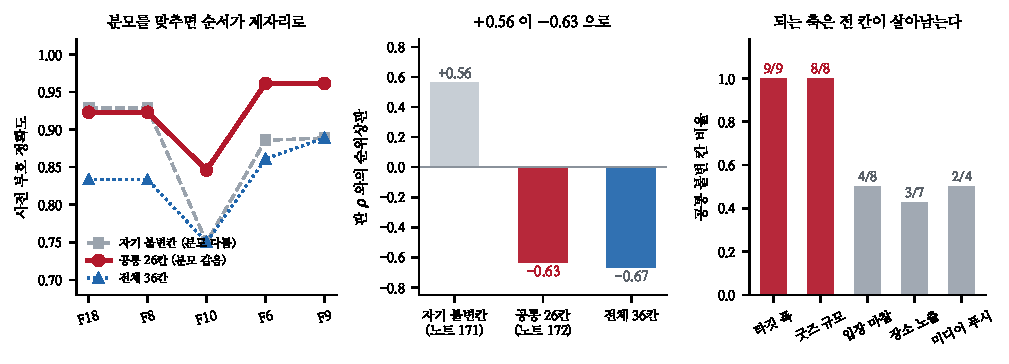
\includegraphics[width=\textwidth]{figs/fair.pdf}
\caption{왼쪽 --- 분모를 맞추면 순서가 제자리로. 가운데 --- $+$0.56이
$-$0.63으로. 오른쪽 --- 되는 축은 전 칸이 살아남는다.}
\end{figure*}

\section{조건화가 맞았다}

\begin{table}[t]
\centering\tsize
\caption{같은 26칸으로 채점. 다섯 정식화가 모두 불변인 칸.}
\begin{tabular}{lrrrr}
\toprule
& 판 $\rho$ & \textbf{공통 26} & 전체 36 & 자기 불변 \\
\midrule
F18 배깅 & \textbf{$+$.4491} & 92\% & 83\% & 93\% \\
F8 부스팅 & $+$.4341 & 92\% & 83\% & 93\% \\
F10 수축 & $+$.3735 & 85\% & 75\% & 75\% \\
F6 능형 & $+$.3671 & \textbf{96\%} & 86\% & 89\% \\
F9 순위우도 & $+$.3519 & \textbf{96\%} & 89\% & 89\% \\
\bottomrule
\end{tabular}
\end{table}

\claimx{\textbf{$+$0.564가 $-$0.632로 돌아온다.} 분모를 맞추자 노트 171의
뒤집힘이 사라지고 다른 잣대 셋과 같은 방향이 된다.}{자기 불변칸 열은
정식화마다 분모가 28$\sim$36으로 달랐다. \textbf{필터가 채점 대상에
따라 달라지면 그 채점은 비교가 아니다} --- 노트 82 · 90의 분모 규칙이
여기에도 걸린다.}

\claimx{\textbf{씨앗을 바꿔도 순위가 똑같다}($+$1.000). 순서 자체는
잡음이 아니다.}{그런데 폭이 0.115이고 26칸 $2\,\mathrm{se}$ 가 0.118이다
--- \textbf{바로 아래다.} 노트 162가 ``칸이 모자라다''고 한 벽이 그대로다.}

\section{26칸이 지난 결론을 재현한다}

\begin{table}[t]
\centering\tsize
\caption{공통 불변 칸의 구성.}
\begin{tabular}{lrr}
\toprule
& 살아남은 칸 & \\
\midrule
\textbf{타깃 폭} & \textbf{9/9} & 전부 \\
\textbf{굿즈 규모} & \textbf{8/8} & 전부 \\
입장 마찰 & 4/8 & 절반 \\
장소 노출 & 3/7 & 절반 아래 \\
미디어 푸시 & 2/4 & 절반 \\
\bottomrule
\end{tabular}
\end{table}

\claimx{\textbf{라벨도 사전 부호도 안 보고 같은 둘이 나온다.} 걸음 다섯
$\times$ 정식화 다섯에서 부호가 한 번도 안 바뀐 칸만 남겼는데, 타깃 폭과
굿즈 규모가 전 칸 통과하고 나머지 셋은 절반이 떨어진다.}{노트 163은
크기로, 164는 구성물 수로, 170은 걸음 불변으로 같은 둘을 지목했다.
\textbf{네 번째 독립 근거이고 이번 것이 제일 약한 가정을 쓴다} --- 상식도
안 쓴다.}

\section{흐름을 닫는다 --- 노트 155$\sim$172}

\begin{table}[t]
\centering\tsize
\caption{열여덟 노트에서 만든 잣대와 잡은 오류.}
\begin{tabular}{ll}
\toprule
\textbf{잣대} & \\
144 귀착 & 남의 축을 흔들면 내 예측이 남나 \\
146 씨앗 & 씨앗을 바꾸면 예측이 남나 \\
147 짝 분해능 & 두 정식화를 가르는 데 드는 차 \\
159 손잡이 & 축을 올리면 옳은 쪽으로 가나 \\
170 걸음 불변 & 걸음을 바꿔도 같은 답인가 \\
172 공통 칸 & 분모를 맞춘 채점 \\
\midrule
\textbf{오류} & \\
156 & 순위 출력에 평균 차를 물었다 \\
160 & 라벨로 정한 방향에 원 부호를 댔다 \\
166 & 복제로 공선성을 만들었다 \\
169 & 열마다 다른 한 칸을 같다고 봤다 \\
171 & 분모가 다른 두 수를 견줬다 \\
\bottomrule
\end{tabular}
\end{table}

\claimx{\textbf{남는 결론 첫째 --- 이 판의 정식화들은 손잡이 모형이
아니다.} 모형이 함의하는 개입 효과와 그 도메인의 부분상관 사이 순위상관이
다섯 정식화 전부 $|{\cdot}| \le 0.14$ 다(노트 156). 줄은 세우고 손잡이는
못 돌린다.}{``맞다''가 아니라 ``자료와도 안 맞는다''까지다 --- 부분상관도
인과가 아니다.}

\claimx{\textbf{남는 결론 둘째 --- 그럼에도 축 둘은 믿을 수 있다.} 타깃
폭과 굿즈 규모는 잣대 여섯 · 정식화 다섯 · 도메인 아홉에서 한 번도 안
틀렸다. \textbf{기획자에게 ``타깃을 넓혀라'' 와 ``굿즈를 키워라''는 말할
수 있다.}}{크기는 여전히 못 말한다(노트 169) --- 한 걸음이 얼마인지가
도메인마다 안 정해져 있다.}

\begin{table}[t]
\centering\tsize
\caption{남은 것.}
\begin{tabular}{ll}
\toprule
칸 & 26$\sim$36으로는 정식화를 못 가른다 --- 벽 그대로 \\
\textbf{단위} & 도메인마다 ``현실적 한 걸음'' --- 미해결 \\
\textbf{다음} & 이 흐름은 닫는다. 자료 쪽으로 돌아간다 \\
\bottomrule
\end{tabular}
\end{table}

마지막 줄이 판단이다. 열여덟 노트가 손잡이를 재는 법을 세웠고 그 결론이
안정됐다. \textbf{더 재도 칸이 모자라 안 갈린다} --- 노트 162가 60칸을,
163이 그것이 도달 불가임을 쟀다. \textbf{남은 지렛대는 자료다}(노트 148의
결론이기도 하다). 과제 82 --- 시장 레코드를 학습에도 넣어 전이 손실
47\%를 회수하는 것 --- 이 다음이다.

\end{document}
